\subsection{Alignment}

% Mer formellt! Inga anekdoter. Den modell som är implicit i datorprogrammet passar inte vårat data.


At first glance one might think that the best and least biased way of getting order to the reads would be to multialign them for each individual. This problem is fairly hard and we tried a number of well known software like MAFFT \cite{mafft} , Muscle \cite{muscle} and Mosaik \cite{mosaik} but none of the models was suitable for our data. In general these softwares could not handle the problem with indels we had in our data.\\
 
From the nature of the DLA region, described in the introduction, one can assume that some parts of the sequence are highly conserved and thereby probably crucial for the function of the protein product. While other parts of the sequence are very variable which seems to be favourable for detecting foreign substances. As discussed in the previous section we will not allow any frameshift insertions or deletions in this exon since it is probably fatal for the product. We want an algorithm that takes advantage of this knowledge in such a way that when, for example, there is a homopolymeric region it is more favourable to do deletions in the end of the homopolymer than in the beginning, since we have observed that almost all homopolymers of length greater than 3 are to short in our data.\\

Our tool of choise was a dynamic programming algorithm for pairwise global sequence alignment, presented by \emph{Saul B. Needleman} and \emph{Christian D. Wunch} \cite{nw} in the early 1970:s. To use global alignment seems natural here when the sequences are very similar and we assume that they should all be of the same length.\\

The modifications we did was to make a scoring table with a unique score scheeme for each position in the reference, this could be done because we had acces to a fairly large number of reference sequences to base the table on. We call this our \emph{Reference Profile.}\\

% In the origninal version of Needleman-Wunch one uses a score matrix with penalties for the diferent matching types, finally the alignment with the lowest score is the optimal alignment. In our version we have swapped the numbers so if a match is more likely it gets a higher score and the optimal alignment is the one with the highest score. It does not really matter which way one does it, we thought it was easier to think of the problem this way.\\

% Skriv ut målfunktionen

\subsubsection{1. Add the same tags to references that was added to all individuals.}

Since the tags used for identification have been sequenced in the same way as the rest of the region they will also have the same problems with indels and error when reading bases, so it is not a trivial problem to remove the tags (we can not just remove a certain length of each end, or use a regular expression to find a pattern to remove). But it is a trivial task to add them to the reference sequences since we know the exact sequence of the tags (they are constructed). We believe that our alignment algorithm, given a reference sequence and a scoring table, can make a correct alignment, so the easiest way to remove the primers is to first align them and then remove them.

\subsubsection{2. Creating the reference profile}

The sequence we want to use in our alignment is called a reference profile since each position have a distribution between a number of alternative nucleotides instead of a static score matrix that is identical for every position. The positions where all reference sequences agree on the same nucleotide are used as `anchors'. We assume that these positions are conserved and therefore we can almost force the algorithm to align correctly against them and be more `loose' in the variable and homopolymeric parts of the sequence.\\

We base our scoring scheme on the frequencies of the nucleotides in each position from the set of reference sequences. Each position also got a fixed negative score for insertion, represented by a gap in the reference sequence, and a fixed negative score for deletion, represented by a gap in the sequence to align. These scores are negative because the indels made by the machine is almost only happening in homopolymers so we do not want to see them in our alignment anywhere else, but they are still allowed.\\

% The exon is 270 base pairs long, we call the positions $n$ where $1\leq n \leq 270$ and the scores $q_a$ where $a\in \{A,C,G,T,Ins,Del\}$.\\

As mentioned earlier, the instrument have problems with homopolymeric sequences and almost allways show to few bases when reading these. To correct for this error we give a positive score for deletions that increases with the length of the homopolymer. This scoring is done in a heuristic fashion based on our observations.

\subsubsection{3. Make a pairwise global sequence alignment with the most abundant reference}

In short, the algorithm walks trough the two sequences and evaluates every possible pair by using a table with different scores for match, mismatch, insertion and deletion. The alignment with the highest score is the optimal alignment with the given score matrix. After alignment we remove all sites where there are gaps in the reference sequence. If our alignment is correct these represents insertions in the sequence to align and according to the asumption made above they are not allowed. No sequence is now longer than the reference sequence but almost all are shorter as a consequence of the deletions from the sequence instrument. Figure \ref{fig:aligned_sequences} show how an aligment of the sequences would look like.

\begin{figure}[ht]
	\centering
		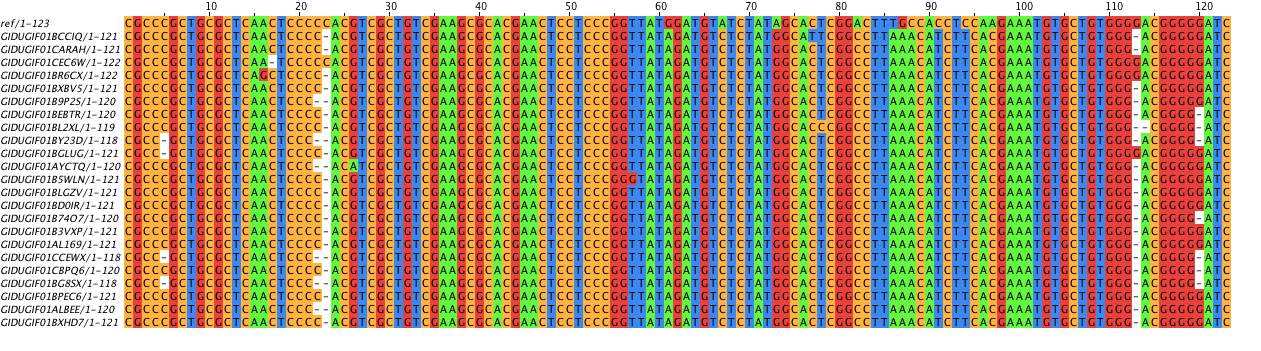
\includegraphics[width=\textwidth]{../pictures/align_with_ref_cropped.png}
	\caption{Aligned sequences with the reference in top.}
	\label{fig:aligned_sequences}
\end{figure}
